\state{Acoustic and optic phonons in the diatomic chain}{
	In the diatomic chain, we take the unit cell to be of length $a$, and take $\xA$ and $\xB$ to be the coordinates of the A and B atoms within the unit cell.  Hence, in the $n$th cell,
	\al{
		\rnA &= n a + \xA; &
		\rnB &= n a + \xB
	}
	\vfix
}

\prob{}{
	In the equations of motion Eq.~(2.30), look for solutions of the form
	\eqn{5a}{
		\unalp = \ealpq \exp( i [ q \rnalp - \omgq t ] ) + \ealpsq \exp( i [-q \rnalp + \omgq t] )
	}
	where $\alp = A$ or $B$, and $\ealp$ are complex numbers that give the amplitude and phase of the oscillation of the two atoms.
	
	Separating out the terms that have the same time dependence, show that (for equal masses, ${\mA = \mB = m}$)
	\al{
		m \omgsq \eAq &= \DAAq \eAq + \DABq \eBq, \\
		m \omgsq \eBq &= \DBAq \eAq + \DBBq \eBq,
	}
	where
	\al{
		\DAAq &= \DBBq = K + K', \\
		-\DABq &= K \exp( i q [ \rnB - \rnA ] ) + K' \exp( i q [ \rnmqB - \rnA ] ), \\
		-\DBAq &= K \exp( i q [ \rnA - \rnB ] ) + K' \exp( i q [ \rnpqA - \rnB ] ).
	}
	Check that $\DAB = \DsBA$.
}

\sol{
	Equation~(2.30) is
	\aln{ \label{thing5a}
		\mA \pdv[2]{\unA}{t} &= K (\unB - \unA) + K' (\unmqB - \unA), &
		\mB \pdv[2]{\unB}{t} &= K' (\unpqA - \unB) + K (\unA - \unB).
	}
	Note that
	\al{
		\pdv[2]{\unalp}{t} &= \pdv{t}\{ -i \omgq \ealpq \exp( i [ q \rnalp - \omgq t ] ) + i \omgq \ealpsq \exp( i [-q \rnalp + \omgq t] ) \} \\
		&= -\omgsq \{ \ealpq \exp( i [ q \rnalp - \omgq t ] ) + \ealpsq \exp( i [-q \rnalp + \omgq t] ) \} \\
		&= -\omgsq \unalp,
	}
	so the first of Eq.~\refeq{5a} can be written
	\al{
		[ K + K' - \mA \omgsq ] \unA &= K \unB + K' \unmqB, \\[1ex]
		&= K \eBq e^{i q \rnB} e^{-i \omgq t} + K \eBsq e^{-i q \rnB} e^{i \omgq t} + K' \eBq e^{i q \rnmqB} e^{-i \omgq t} \\
		&\hspace{5em} \phantom{=\ } + K' \eBsq e^{-i q \rnmqB} e^{i \omgq t} \\[1ex]
		&= K \eBq e^{i q [ na + \xB ]} e^{-i \omgq t} + K' \eBq e^{i q [ (n - 1) a + \xB ]} e^{-i \omgq t} + K \eBsq e^{-i q [ na + \xB ]} e^{i \omgq t} \\
		&\hspace{5em} \phantom{=\ } + K' \eBsq e^{-i q [ (n - 1) a + \xB ]} e^{i \omgq t} \\[1ex]
		&= (K + e^{-i q a} K') \eBq e^{i q (na + \xB)} e^{-i \omgq t} + (K + e^{-i q a} K') \eBsq e^{-i q (na + \xB)} e^{i \omgq t} \\[1ex]
		&= (K + e^{-i q a} K') \unB.
	}
	Generalizing this, we have
	\al{
		[ K + K' - \mA \omgsq ] \unA &= (K + e^{-i q a} K') \unB, &
		[ K + K' - \mB \omgsq ] \unB &= (K + e^{i q a} K') \unA.
	}
	
	Collecting terms of like time dependence yields
	\aln{
		[ K + K' - m \omgsq ] \eAq e^{i q \rnA} &= (K + e^{-i q a} K') \eBq e^{i q \rnB}, \label{thing5.a1} \\
		[ K + K' - m \omgsq ] \eBq e^{i q \rnB} &= (K + e^{i q a} K') \eAq e^{i q \rnA}, \label{thing5.a2}
	}
	for $e^{-i \omg t}$, and
	\al{
		[ K + K' - m \omgsq ] \eAsq e^{-i q \rnA} &= (K + e^{-i q a} K') \eBsq e^{-i q \rnB}, \\
		[ K + K' - m \omgsq ] \eBsq e^{-i q \rnB} &= (K + e^{-i q a} K') \eAsq e^{-i q \rnA}.
	}
	for $e^{i \omg t}$.
	
	Rearranging Eqs.~\refeq{thing5.a1} and \refeq{thing5.a2}, we have
	\al{
		m \omgsq \eAq &= (K + K') \eAq - (K + e^{-i q a} K') e^{i q (\rnB - \rnA)} \eBq \\
		&= (K + K') \eAq - (e^{i q (\rnB - \rnA)} K + e^{i q (\rnmqB - \rnA)} K') \eBq, \\[1ex]
		m \omgsq \eBq &= -(K + e^{i q a} K') e^{i q (\rnA - \rnB)} \eAq - (K + K') \eBq \\
		&= -(e^{i q (\rnA - \rnB)} K + e^{i q (\rnpqA - \rnB)} K') \eAq - (K + K') \eBq,
	}
	which gives us
	\ans{ \al{
		\DAAq &= \DBBq = K + K', \\
		\DABq &= -e^{i q (\rnB - \rnA)} K - e^{i q (\rnmqB - \rnA)} K', \\
		\DBAq &= -e^{i q (\rnA - \rnB)} K - e^{i q (\rnpqA - \rnB)} K',
	}}%
	as we wanted to show. \qed
	
	Finally, note that
	\al{
		\DsBA &= [ -e^{i q (\rnA - \rnB)} K - e^{i q (\rnpqA - \rnB)} K' ]^*
		= -e^{i q (\rnB - \rnA)} K - e^{i q (\rnB - \rnpqA)} K' \\
		&= -e^{i q (\rnB - \rnA)} K - e^{i q (\rnB - \rnA)} e^{-i q a} K'
		= -e^{i q (\rnB - \rnA)} K - e^{i q (\rnmqB - \rnA)} K' \\
		&= \ans{ \DAB }
	}
	as desired. \qed
}



\prob{}{
	The $2 \times 2$ matrix equation can have a nontrivial solution if the determinant vanishes:
	\eq{
		\mqty| 	\DAAq - m \omgsq & \DABq \\
				\DBAq & \DBBq - m \omgsq |
		= 0.
	}
	Hence show that the frequencies of the modes are given by
	\eq{
		m \omgsq = K + K' \pm \sqrt{ (K + K')^2 - 4 K K' \sin[2]( \frac{q a}{2} ) }.
	}
	\vfix
}

\sol{
	The determinant is
	\eq{
		0 = [ \DAAq - m \omgsq ] [ \DBBq - m \omgsq ] - \DABq \DBAq
		= [ \DAAq - m \omgsq ]^2 - \DABq \DBAq,
	}
	which implies
	{\allowdisplaybreaks
	\aln{
		m \omgsq &= \DAAq \pm \sqrt{\DABq \DBAq} \notag \\
		&= K + K' \pm \sqrt{(e^{i q (\rnB - \rnA)} K + e^{i q (\rnmqB - \rnA)} K') (e^{i q (\rnA - \rnB)} K + e^{i q (\rnpqA - \rnB)} K')} \notag \\
		&= K + K' \pm \sqrt{(K + e^{-i q a} K') e^{i q (\rnB - \rnA)} (K + e^{i q a} K') e^{i q (\rnA - \rnB)}} \notag \\
		&= K + K' \pm \sqrt{(K + e^{-i q a} K') (K + e^{i q a} K')}
		= K + K' \pm \sqrt{K^2 + (e^{i q a} + e^{-i q a}) K K' + {K'}^2} \notag \\
		&= K + K' \pm \sqrt{K^2 + 2\cos(q a) K K' + {K'}^2} \label{5bo} \\
		&= K + K' \pm \sqrt{K^2 + \brac{ 2 - 4 \sin[2](\frac{q a}{2}) } K K' + {K'}^2} \notag \\
		&= K + K' \pm \sqrt{K^2 + 2 K K' + {K'}^2 - 4 \sin[2](\frac{q a}{2}) K K'} \notag \\
		&= \ans{ K + K' \pm \sqrt{ (K + K')^2 - 4 K K' \sin[2]( \frac{q a}{2} ) }, } \label{5b}
	}}
	where we have used the double-angle formula $\cos(2x) = 1 - 2 \sin[2](x)$~\cite{DoubleAngle}. \qed
}



\prob{}{
	Sketch the dispersion relations when $K / K' =  2$.
}

\sol{
	There are two dispersion curves since there are two solutions in Eq.~\refeq{5b}.  The expressions for the branches are
	\eqn{5ceq}{
		\omgq = \frac{1}{\sqrt{m}} \sqrt{ K + K' \pm \sqrt{ (K + K')^2 - 4 K K' \sin[2]( \frac{q a}{2} ) } }
		\begin{cases}
			\text{optical}, \\
			\text{acoustic},
		\end{cases}
	}
	where the acoustic~(optical) branch corresponds to the upper~(lower) sign.  Both branches are shown in Fig.~\ref{5c}, with the $K / K' =  2$ case on the left and the $K = K'$ case on the right.
	
	\fig{5c}{
		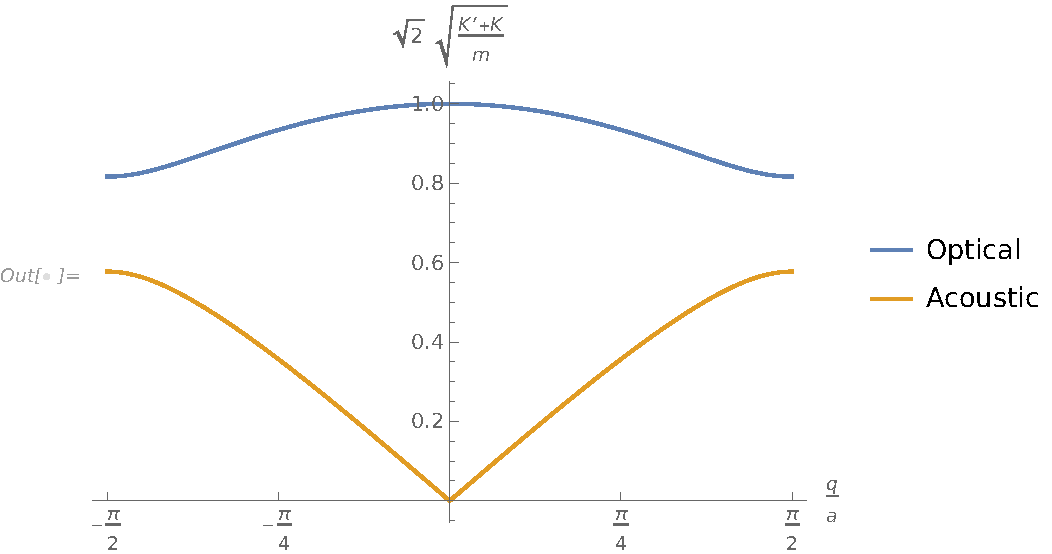
\includegraphics[width=0.5\textwidth,trim=1.5cm 0 0 0,clip]{5c}
		\caption{Dispersion curves for $K / K' =  2$.  The optical branch~(blue) corresponds to the upper sign in Eq.~\refeq{5ceq}, and the acoustic branch~(gold) to the lower sign.}
	}
}



\prob{}{
	  Discuss what happens if $K = K'$.
}

\sol{
	If $K = K'$, then not only are the masses of the two atoms identical, but so are their restorative forces.  Thus, the system is essentially reduced to a monatomic chain~\cite[p.~437]{Ashcroft}.  Picking up from Eq.~\refeq{5bo},
	\eq{
		m \omgsq = 2 K \pm \sqrt{2 K^2 + 2 \cos(q a) K^2}
		= 2 K \pm K \sqrt{4 \cos[2](\frac{q a}{2})}
		= 2 K \brac{ 1 - \cos(\frac{q a}{2}) }
		= 4 K \sin[2](\frac{q a}{4}),
	}
	where we have used the double-angle formula $\cos(2 x) = 2 \cos[2](x) - 1$~\cite{DoubleAngle}.  This is Eq.~\refeq{2.25} with $q a \to q a / 2$.  So in this limit, the diatomic chain is reduced to a monatomic chain with lattice constant $a / 2$~\cite[p.~437]{Ashcroft}.
}